\documentclass[11pt]{article}

% ---------- Packages ----------
\usepackage[margin=0.9in]{geometry}
\usepackage[T1]{fontenc}
\usepackage{lmodern}
\usepackage{microtype}
\usepackage{booktabs}
\usepackage{array}
\usepackage{tabularx}
\newcolumntype{L}[1]{>{\raggedright\arraybackslash}p{#1}}
\usepackage{longtable}
\usepackage{colortbl}
\usepackage[table]{xcolor}
\usepackage{enumitem}
\usepackage{fancyhdr}
\usepackage{titlesec}
\usepackage{tikz}
\usetikzlibrary{positioning}
\usepackage{pgfplots}
\pgfplotsset{compat=1.16}
\usepackage[breakable,skins]{tcolorbox}
\usepackage[hidelinks]{hyperref}
\usepackage{xurl}

% ---------- Colours ----------
\definecolor{civic}{HTML}{2E6FBF}
\definecolor{robo}{HTML}{8E44AD}
\definecolor{clim}{HTML}{1E8449}
\definecolor{health}{HTML}{C0392B}
\definecolor{okgreen}{HTML}{1E8449}
\definecolor{warnorange}{HTML}{D35400}
\definecolor{badred}{HTML}{B03A2E}
\definecolor{greyish}{HTML}{7F8C8D}
\definecolor{lightbg}{HTML}{F4F6F7}

% ---------- Status macros ----------
\newcommand{\LIVE}{\textcolor{okgreen}{\textbf{LIVE}}}
\newcommand{\BLOCKED}{\textcolor{warnorange}{\textbf{BLOCKED}}}
\newcommand{\UNTESTED}{\textcolor{greyish}{\textbf{not tested}}}
\newcommand{\LISTED}{\textcolor{greyish}{\textbf{listed only}}}
\newcommand{\tagC}{\textcolor{civic}{\textbf{Civic}}}
\newcommand{\tagR}{\textcolor{robo}{\textbf{Robotics}}}
\newcommand{\tagE}{\textcolor{clim}{\textbf{Climate}}}
\newcommand{\tagH}{\textcolor{health}{\textbf{Health}}}
\newcommand{\yes}{\textcolor{okgreen}{\textbf{$\bullet$}}}

% ---------- Layout ----------
\setlist{nosep,leftmargin=1.2em}
\setlength{\parindent}{0pt}
\setlength{\parskip}{0.45em}
\renewcommand{\arraystretch}{1.18}
\pagestyle{fancy}
\fancyhf{}
\lhead{\small Hackachusetts 2026 -- Research Review}
\rhead{\small Round 3, 24 Oct 2026}
\cfoot{\thepage}
\titleformat{\section}{\Large\bfseries}{\thesection}{0.6em}{}
\titleformat{\subsection}{\large\bfseries}{\thesubsection}{0.5em}{}

% ---------- Idea card box ----------
\newtcolorbox{ideacard}[2]{%
  breakable, enhanced, colback=white, colframe=#1, coltitle=white,
  fonttitle=\bfseries\large, title={#2}, boxrule=0.9pt, arc=2pt,
  left=6pt, right=6pt, top=4pt, bottom=4pt, before skip=10pt, after skip=10pt}
\newtcolorbox{notebox}[1][]{%
  breakable, enhanced, colback=lightbg, colframe=greyish, boxrule=0.5pt,
  arc=2pt, left=6pt, right=6pt, top=4pt, bottom=4pt, #1}

\newcommand{\field}[1]{\textbf{\textsf{#1}}\quad}

\begin{document}

% =====================================================================
\begin{titlepage}
\centering
\vspace*{2cm}
{\Huge\bfseries Hackachusetts 2026\par}
\vspace{0.4cm}
{\LARGE Project research: what we found and what we recommend\par}
\vspace{1.2cm}
{\large Saturday 24 October 2026 \quad$\cdot$\quad Build day: 09:00--20:00 (about 11 hours)\par}
\vspace{1.5cm}
\begin{notebox}[width=0.85\textwidth]
\textbf{What this document is.} One place to review all the research: what the
event actually asks for, the datasets it gives us, how ideas were picked and dropped, the top
five ideas with build plans, and the decisions the team has to make tonight.

\textbf{How much to trust it.} Every dataset marked \LIVE{} was fetched by
\texttt{curl} on 24 Oct 2026 and returned real data. Items marked \LISTED{} appear in the
official portal but were \emph{not} fetched. URLs in the evidence tables from earlier rounds
were spot-checked; quotes labelled \emph{verified} were seen word for word. Anything else
should be checked before you rely on it.

\textbf{Source of truth.} The workspace \texttt{\textasciitilde/research/}
(\texttt{00\_INDEX.md}, \texttt{40\_shortlist.md}, \texttt{90\_log.md}, \texttt{20\_findings/},
\texttt{30\_candidates/}). This PDF is a readable summary of those files.
\end{notebox}
\vfill
{\small Prepared for a 6-person team: 4 CS undergrads, 1 math grad student (spec writer),
1 chemistry major. Laptops only, free public data, one LLM coding agent.\par}
\end{titlepage}

\tableofcontents
\newpage

% =====================================================================
\section{Executive summary}

\textbf{Bottom line.} Earlier research used the wrong track list and never used the official
data portal. Under the real tracks, the earlier top three (Mass Save rebates, FRC mentor
logging, FRC inspection) fall out. The new top five are built on the portal's datasets,
each one maps to a named challenge, and together they cover all four tracks.

\begin{longtable}{@{}c L{5.2cm} L{1.7cm} c c c L{6.0cm}@{}}
\toprule
\textbf{\#} & \textbf{Idea} & \textbf{Track} & \textbf{I} & \textbf{F} & \textbf{N} & \textbf{Why it ranks here}\\
\midrule
\endhead
1 & \textbf{311 triage}: repeat reports \& missed deadlines in Boston 311, with an equity overlay & \tagC & 4 & 4 & 4 & Uses the exact columns the challenge names; real city data; a resident can actually use the demo.\\
2 & \textbf{Bridge triage}: maintenance priority list from MA bridge-inspection data & \tagR & 3 & 4 & 4 & Matches the challenge wording (the bottleneck is now interpretation); clean static file.\\
3 & \textbf{Path-planner classifier}: which algorithm to use for a given map & \tagR & 3 & 5 & 4 & Safest build (pure Python, offline). Backup if a data-heavy idea stalls.\\
4 & \textbf{Emergency outreach}: which neighbourhoods get missed in a flood & \tagC & 4 & 4 & 4 & Strong equity angle on 3 live datasets; has a reliable fallback mode.\\
5 & \textbf{Trial finder}: MA clinical trials in plain language, by distance & \tagH & 3 & 4 & 3 & Clean, safe build on a live federal feed; gives us a Healthcare entry.\\
\bottomrule
\end{longtable}

{\small I = impact, F = feasibility in 11 h, N = novelty / how under-served the problem is. All scores are 1--5.}

\textbf{Beyond the top five:} Section~\ref{sec:inspo} gives \textbf{8 more ideas} (an MBTA step-free route checker, a robot-data linter, swarm search-and-rescue, a MassHealth notice decoder, and others). They are less researched, but several have the same live data behind them.

\textbf{Decisions needed tonight} (details in Section~\ref{sec:questions}):
\begin{enumerate}
\item Choose \textbf{one} idea, or two at most. With 6 people and 11 hours, two ideas is already a stretch.
\item If it is \#1: download a Boston 311 data slice \emph{tonight}. The city site blocks
  server-side downloads (Cloudflare).
\item Install-test the libraries on every laptop tonight (PythonRobotics, Leaflet, pandas).
\item Decide whether to focus on one track (Civic is the most open) or spread across tracks.
\end{enumerate}

% =====================================================================
\section{What the event actually asks for}

\subsection{Where this comes from}
The site \url{https://hackachusetts2026.vercel.app/} renders in the browser, so normal
page fetchers return a blank page. We downloaded its JavaScript bundle and pulled out the
track, challenge, and dataset definitions directly. The event's own guidance says:
\emph{``These are not the final ideas on each track. They are just for guidance.''}
Two pages linked from the site (the coalition event page and a Notion rules page) also render
in the browser and could \textbf{not} be read. \textbf{Read the judging criteria and team
rules in a browser tonight.}

\subsection{The four real tracks}
\begin{longtable}{@{}L{3.4cm} L{5.2cm} L{6.4cm}@{}}
\toprule
\textbf{Track} & \textbf{Official one-liner} & \textbf{Correction to earlier research}\\
\midrule
\endhead
\tagH{} --- Healthcare \& biotech & Turn continuous data, coverage, and research into better care. & Roughly matches the old ``Healthtech/Biotech''. Note that it puts weight on wearables, MassHealth coverage, and access, not only lab biotech.\\
\tagR{} --- Robotics \& hardware & Bring intelligence into the physical world. & The challenges are about physical AI: automation, simulation, data quality, inspection, planning. Youth-team logistics (the FRC ideas) do not fit this.\\
\tagE{} --- Energy \& climate tech & Tackle how we power our world and protect our planet. & Was ``Energy''. Climate resilience, the ocean, and the coastal economy are also in scope.\\
\tagC{} --- Civic action & Strengthen the places, communities, and opportunities that shape daily life. & \textbf{New.} There is \textbf{no Education track}; education and college ideas belong here.\\
\bottomrule
\end{longtable}

\subsection{All 20 challenge statements, and which ideas address them}
Columns: \textbf{1}=311 triage, \textbf{2}=bridge triage, \textbf{3}=path planner,
\textbf{4}=emergency outreach, \textbf{5}=trial finder, \textbf{P}=a parked idea covers it.
Empty rows are challenges \emph{nobody on our list addresses yet}. Those are open
opportunities, but they were not researched this session.

\begin{longtable}{@{}L{1.6cm} L{8.3cm} c c c c c c@{}}
\toprule
\textbf{Track} & \textbf{Challenge (summary of the official text)} & \textbf{1} & \textbf{2} & \textbf{3} & \textbf{4} & \textbf{5} & \textbf{P}\\
\midrule
\endhead
\tagC & \textbf{Better Together}: everyday problems with housing, transport, public space, community, opportunity &&&&&&\\
\tagC & \textbf{Citizen-Friendly Digital Government}: complex websites, long PDFs, language barriers, confusing applications &&&&&& \yes\\
\tagC & \textbf{More Responsive Neighborhood Services}: 311 volume, repeat reports, prioritizing, reporting progress & \yes &&&&&\\
\tagC & \textbf{Stronger Community Emergency Readiness}: fast-changing information; vulnerable people are hardest to reach &&&& \yes &&\\
\tagE & \textbf{Resilient communities in a changing climate}: heat, flooding, storms; risk differs by neighbourhood &&&& \yes && \yes\\
\tagE & \textbf{Cleaner, more affordable buildings}: old buildings, retrofit cost, uneven program access &&&&&& \yes\\
\tagE & \textbf{A more reliable clean energy system}: peaks, severe weather, adding renewables, cost &&&&&& \yes\\
\tagE & \textbf{Understanding and protecting the ocean}: combining vessel, buoy, glider, and satellite data &&&&&&\\
\tagE & \textbf{Sustainable blue economy}: fishing, aquaculture, shipping, offshore wind sharing the same water &&&&&&\\
\tagH & \textbf{Turning Wearable Data into Better Healthcare}: continuous monitoring into useful insight &&&&&&\\
\tagH & \textbf{Keeping Residents Connected to Health Coverage}: MassHealth renewal, missed notices, upcoming rule changes &&&&&&\\
\tagH & \textbf{Improving Healthcare Access and Coordination}: referrals and scheduling; rural travel distance &&&&&&\\
\tagH & \textbf{Accelerating Biotechnology Innovation}: AI for research and experiments &&&&&& \yes\\
\tagH & \textbf{Making Clinical Research More Accessible}: finding trials; technical eligibility text; language, distance &&&&&\yes&\\
\tagR & \textbf{Making Automation Accessible to Manufacturers}: small shops lack the staff and capital &&&&&&\\
\tagR & \textbf{Robo-Gym Training Environments}: simulated real places for physical-AI training &&&&&&\\
\tagR & \textbf{Real-Time Control for Data Quality}: catching bad robot-training data during collection &&&&&&\\
\tagR & \textbf{Swarm Robotics for Search-and-Rescue}: coordination, mapping, task allocation &&&&&&\\
\tagR & \textbf{Safer Inspection of Critical Infrastructure}: MassDOT already flies drones; interpreting what they capture is now the bottleneck && \yes &&&&\\
\tagR & \textbf{Path Planning Classifier}: pick a planning algorithm for the environment and compute budget &&& \yes &&&\\
\bottomrule
\end{longtable}

The portal also groups civic datasets under five extra headings: \emph{Simplified public
services, Responsive and resilient communities, Safer and connected places, Better college
experiences, Pathways to education and opportunity.} The last two are where former
``education'' ideas would go.

% =====================================================================
\section{How ideas were selected}

\subsection{What changed from earlier rounds}
\begin{enumerate}
\item \textbf{Wrong tracks.} Rounds 1--2 assumed Healthtech, Robotics, Energy, Education.
\item \textbf{Ignored the portal.} The event provides 166 datasets and resources, chosen for
  each challenge. None of the earlier top picks used any of them. In a hackathon built
  around a data portal, judges will look for honest use of that data.
\item \textbf{Too focused on single individuals.} Earlier gates required a dated forum post
  from one named person and dropped any idea with 3 or more competitors. Following your
  steer, the target is now \emph{real problems that real people and organizations have, which
  existing tools solve poorly or not at all}. Evidence can be a government program, a
  documented structural gap, or the challenge text itself.
\end{enumerate}

\subsection{Gates: old vs.\ new}
\begin{longtable}{@{}L{2.6cm} L{6.0cm} L{6.4cm}@{}}
\toprule
\textbf{Gate} & \textbf{Rounds 1--2} & \textbf{Round 3}\\
\midrule
\endhead
Real & Dated first-person complaint required & Documented real-world problem: challenge text, government program, data, or practitioner traces\\
Buildable & 11 h, laptops, LLM agent & Same, plus the data must download from \emph{our} laptops tonight\\
Under-served & 3+ competitors means dropped & Existing tools serve it \emph{poorly}; competition is a warning, not an automatic drop\\
Track fit & Old 4 tracks & Real 4 tracks \textbf{and} a named challenge\\
Uses portal & (not checked) & \textbf{New:} provided MA datasets do the real work in the build, not just decoration\\
Safe & No health PII, no advice, etc. & Same; also no auto-written official messages\\
Demo & A 60-second before/after & Same, plus a cached fallback so the demo can't hang\\
\bottomrule
\end{longtable}

\subsection{Pipeline at a glance}
\begin{center}
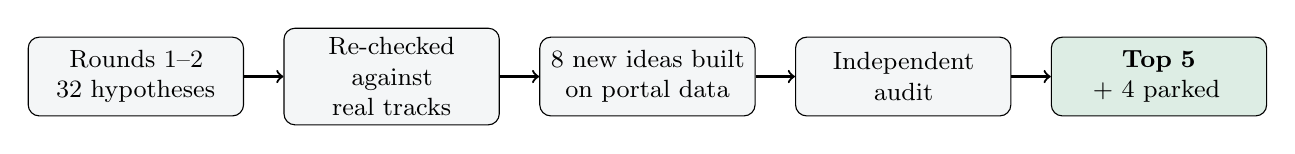
\begin{tikzpicture}[node distance=0.35cm and 0.5cm, every node/.style={font=\small},
  box/.style={draw, rounded corners, align=center, minimum height=1.0cm, text width=2.5cm, fill=lightbg}]
\node[box] (a) {Rounds 1--2\\32 hypotheses};
\node[box, right=of a] (b) {Re-checked against real tracks};
\node[box, right=of b] (c) {8 new ideas built on portal data};
\node[box, right=of c] (d) {Independent audit};
\node[box, right=of d, fill=okgreen!15] (e) {\textbf{Top 5}\\+ 4 parked};
\draw[->, thick] (a) -- (b); \draw[->, thick] (b) -- (c);
\draw[->, thick] (c) -- (d); \draw[->, thick] (d) -- (e);
\end{tikzpicture}
\end{center}

% =====================================================================
\section{Score comparison}

\begin{center}
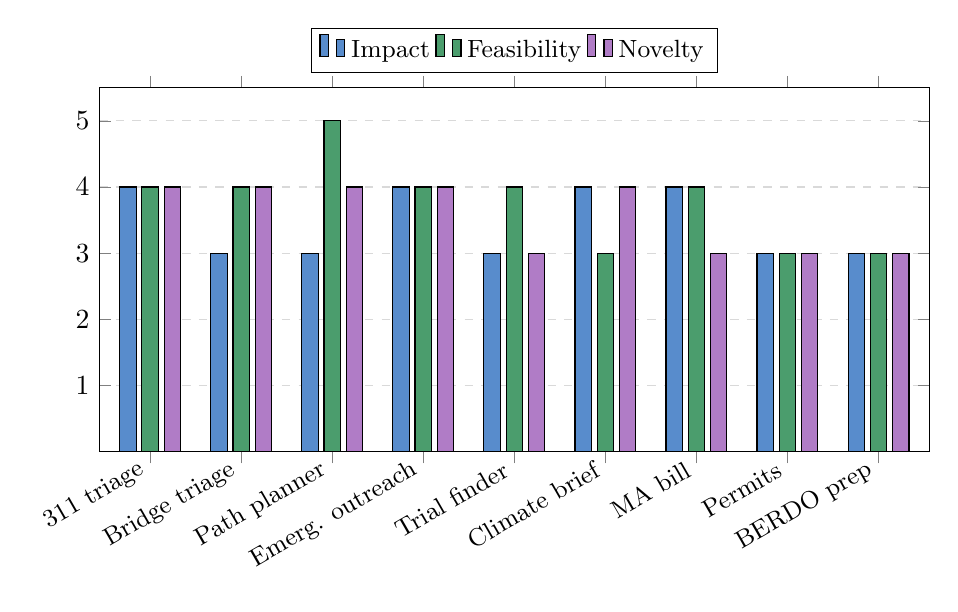
\begin{tikzpicture}
\begin{axis}[
  ybar, bar width=6pt, width=\textwidth, height=6.2cm,
  ymin=0, ymax=5.5, ytick={1,2,3,4,5},
  symbolic x coords={311 triage,Bridge triage,Path planner,Emerg. outreach,Trial finder,Climate brief,MA bill,Permits,BERDO prep},
  xtick=data, x tick label style={rotate=30, anchor=east, font=\small},
  legend style={at={(0.5,1.04)}, anchor=south, legend columns=3, font=\small},
  ymajorgrids, grid style={dashed,gray!30}, enlarge x limits=0.07]
\addplot[fill=civic!80] coordinates {(311 triage,4) (Bridge triage,3) (Path planner,3) (Emerg. outreach,4) (Trial finder,3) (Climate brief,4) (MA bill,4) (Permits,3) (BERDO prep,3)};
\addplot[fill=clim!80] coordinates {(311 triage,4) (Bridge triage,4) (Path planner,5) (Emerg. outreach,4) (Trial finder,4) (Climate brief,3) (MA bill,4) (Permits,3) (BERDO prep,3)};
\addplot[fill=robo!70] coordinates {(311 triage,4) (Bridge triage,4) (Path planner,4) (Emerg. outreach,4) (Trial finder,3) (Climate brief,4) (MA bill,3) (Permits,3) (BERDO prep,3)};
\legend{Impact, Feasibility, Novelty}
\end{axis}
\end{tikzpicture}
\end{center}
The first five are the shortlist; the last four are parked. Scores are judgment calls from
the evidence, not measurements. Ties are broken by how much the idea relies on portal data
and how reliable its demo is.

\begin{center}
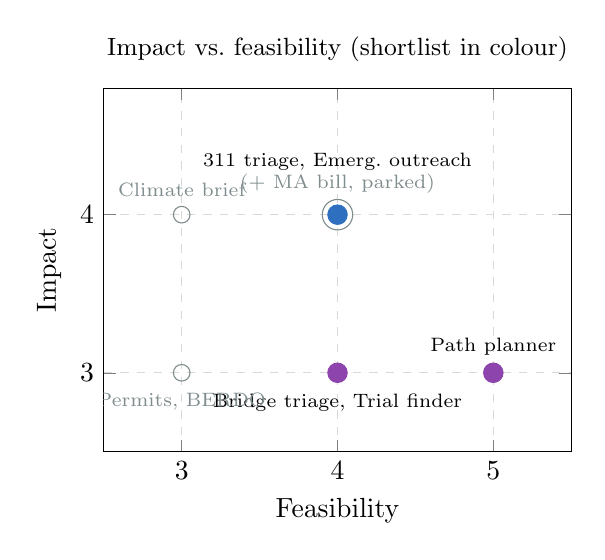
\begin{tikzpicture}
\begin{axis}[width=0.62\textwidth, height=6.2cm, xmin=2.5, xmax=5.5, ymin=2.5, ymax=4.8,
  xlabel={Feasibility}, ylabel={Impact}, xtick={3,4,5}, ytick={3,4},
  grid=both, grid style={dashed,gray!30}, title={\small Impact vs.\ feasibility (shortlist in colour)}]
\addplot[only marks, mark=o, mark size=5.5pt, color=greyish] coordinates {(4,4)};
\addplot[only marks, mark=*, mark size=3.5pt, color=civic] coordinates {(4,4)};
\node[anchor=south, font=\scriptsize, align=center] at (axis cs:4,4.07) {311 triage, Emerg.\ outreach\\\textcolor{greyish}{(+ MA bill, parked)}};
\addplot[only marks, mark=*, mark size=3.5pt, color=robo] coordinates {(4,3) (5,3)};
\node[anchor=north, font=\scriptsize, align=center] at (axis cs:4,2.93) {Bridge triage, Trial finder};
\node[anchor=south, font=\scriptsize] at (axis cs:5,3.05) {Path planner};
\addplot[only marks, mark=o, mark size=3pt, color=greyish] coordinates {(3,4) (3,3)};
\node[anchor=south, font=\scriptsize, text=greyish] at (axis cs:3,4.05) {Climate brief};
\node[anchor=north, font=\scriptsize, text=greyish] at (axis cs:3,2.93) {Permits, BERDO};
\end{axis}
\end{tikzpicture}
\end{center}

% =====================================================================
\section{The shortlist: full idea cards}

% ---------------- 1 ----------------
\begin{ideacard}{civic}{\#1 \quad 311 triage --- repeat reports and missed deadlines, with an equity overlay}
\field{Track / challenge} \tagC{} --- More Responsive Neighborhood Services (311)\par
\field{Scores} I4 F4 N4

\field{Problem} The challenge itself says: \emph{``high volumes and repeated reports can make
it hard to recognize patterns, prioritize action, and communicate progress.''} Duplicate
reports of the same pothole inflate the counts and hide problems that never get fixed.
Residents cannot tell whether their block is routinely ignored. Typical 311 dashboards show
volume. They do not merge duplicates or show where missed deadlines cluster.

\field{Who it helps} City operations staff (prioritizing work) and residents and councillors
(seeing chronic neglect).

\field{Data}
\begin{itemize}
\item Boston 311 requests: \texttt{service\_name}, \texttt{case\_status}, \texttt{on\_time},
  \texttt{neighborhood}, \texttt{ward}, \texttt{open\_date} --- \BLOCKED{} for server-side
  \texttt{curl} (Cloudflare). Should work from a browser. \textbf{Download a slice tonight.}
\item MassGIS environmental-justice block groups (minority \%, limited-English \%, median
  income) --- \LIVE.
\end{itemize}

\field{Demo (60 s)} Pick a neighbourhood. A map shows open cases and cases that missed their
deadline. Duplicate pothole reports collapse into one hot spot. The top three chronic
categories are listed. An overlay shows that missed deadlines concentrate in a
limited-English block group.

\field{Hardest steps} (1) Getting the data past Cloudflare. (2) A duplicate rule (same
service, nearby, close in time) that doesn't merge unrelated reports. (3) An equity claim that
holds up after normalizing for report volume.

\field{Build plan}\par\nopagebreak
\begin{tabularx}{\linewidth}{@{}L{1.2cm} X@{}}
09:00 & Math grad writes the spec: duplicate rule, ``missed'' means \texttt{on\_time} is false, per-capita normalization. Data slice must already be cached.\\
10:00 & CS1+CS2: load data and cluster duplicates. CS3: Leaflet map. CS4: join to EJ block groups.\\
13:00 & Chem major (tester): check clusters and counts against the raw rows.\\
15:00 & Chronic-category ranking and a one-line summary for residents.\\
16:30 & Rehearse the demo story. \textbf{18:00 freeze} on cached data.\\
\end{tabularx}

\field{Risks / fallback} If the live download fails, the cached slice is the demo (plan for
this from the start). If the duplicate rule merges wrong reports, show the raw rows behind
every cluster. If the equity pattern isn't there, report what the data actually shows; that
is still a useful tool.
\end{ideacard}

% ---------------- 2 ----------------
\begin{ideacard}{robo}{\#2 \quad Bridge triage --- maintenance priorities from MA bridge-inspection data}
\field{Track / challenge} \tagR{} --- Safer Inspection of Critical Infrastructure\par
\field{Scores} I3 F4 N4

\field{Problem} The challenge says MassDOT Aeronautics \emph{already flies drones} to inspect
bridges, and \emph{``the bottleneck has moved''} from capturing data to interpreting it. The
National Bridge Inventory (NBI) is a wall of coded columns. A ranked, explained
``which bridges need attention, and why'' list is the interpretation step the challenge
asks for.

\field{Who it helps} State and municipal bridge asset managers and inspection planners.

\field{Data}
\begin{itemize}
\item NBI Massachusetts file (\texttt{MA22.txt}) --- \LIVE, real condition columns.
\item FHWA InfoBridge and the new SNBI schema docs --- \LISTED{} (needed to decode the columns).
\item dacl10k bridge-defect images (Hugging Face) --- \LIVE{} (metadata API); CODEBRIM --- \LISTED.
\end{itemize}

\field{Demo (60 s)} Load the MA NBI file and get a ranked list. Each rank is explained by the
deck, superstructure, and substructure ratings behind it. Click a bridge to see a sample
inspection photo with cracks or corrosion flagged (stretch goal).

\field{Hardest steps} (1) Decoding the NBI items correctly (58 deck, 59 superstructure,
60 substructure); one wrong column produces a confidently wrong ranking. (2) A priority
score you can defend. (3) Optional: running a defect model on the CPU over 5--10 images.

\field{Build plan}\par\nopagebreak
\begin{tabularx}{\linewidth}{@{}L{1.2cm} X@{}}
09:00 & Math grad: column-decoding table checked against the FHWA docs and committed to the repo; scoring rule.\\
10:00 & CS1+CS2: parser, scoring, ranked table. CS3: bridge detail view. CS4: defect model on cached sample images.\\
13:00 & Chem major (tester): spot-check 20 bridges against their raw ratings.\\
15:00 & Connect the image flags, or drop to table-only.\\
16:30 & Rehearse the demo (one county). \textbf{18:00 freeze}.\\
\end{tabularx}

\field{Risks / fallback} Show the decoding table during the demo; that turns the biggest risk
into a point of credibility. Present it as a \emph{maintenance-planning aid}, not a safety
verdict. Be ready to say how it differs from FHWA InfoBridge. Without the images it is still
a complete demo.
\end{ideacard}

% ---------------- 3 ----------------
\begin{ideacard}{robo}{\#3 \quad Path-planner classifier --- ``which algorithm should I use here?''}
\field{Track / challenge} \tagR{} --- Path Planning Classifier\par
\field{Scores} I3 F5 N4

\field{Problem} The challenge text: \emph{``How to choose which path planning algorithm for
your environmental needs and compute resources or other constraints.''} People pick A* or
RRT out of habit. A tool that runs several planners on the same map and recommends one
answers the question directly.

\field{Who it helps} Robotics students and engineers. Of the five, this is the weakest
``real-world problem'' and the least specific to MA. It ranks \#3 because it is very
unlikely to fail.

\field{Data / code}
\begin{itemize}
\item movingai street benchmark maps: \texttt{Boston\_0\_256} --- \LIVE; \texttt{Boston\_1/2},
  NewYork, Berlin also \LIVE{} (enables a multi-map test matrix).
\item Boston street centerlines (19,440 segments, real geometry) --- \LISTED{} (data.boston.gov; same Cloudflare caveat).
\item PythonRobotics (A*, Dijkstra, RRT, PRM in pure Python) --- \LIVE{} (repo reachable).
\end{itemize}

\field{Demo (60 s)} Pick a map, a start, and a goal. A*, Dijkstra, RRT, and PRM race side by
side, showing path length, nodes expanded, and runtime. The classifier recommends one and
says why. Then repeat on the real Boston street graph.

\field{Hardest steps} (1) A recommendation rule learned from \emph{many} maps; one map would
just make it a lookup table. (2) RRT runs vary and can time out. (3) A shared interface over
PythonRobotics scripts, which were written as demos rather than as a library.

\field{Build plan}\par\nopagebreak
\begin{tabularx}{\linewidth}{@{}L{1.2cm} X@{}}
09:00 & Math grad: map features (obstacle density, free-space ratio, size) and the metrics.\\
09:30 & CS1+CS2: wrap the planners behind one interface. CS3: grid UI. CS4: metrics and path overlays.\\
13:00 & Tester: run every map against every planner; fix random seeds and cap iterations.\\
15:00 & Fit the rule from the measured results; add the explanation.\\
16:30 & Rehearse the demo. \textbf{18:00 freeze} with precomputed runs.\\
\end{tabularx}

\field{Risks / fallback} Don't claim ``optimal''; present it as a guided comparison. Even if
the classifier is weak, the side-by-side race works as a demo on its own.
\end{ideacard}

% ---------------- 4 ----------------
\begin{ideacard}{civic}{\#4 \quad Emergency outreach --- who gets missed when a flood is coming}
\field{Track / challenge} \tagC{} --- Stronger Community Emergency Readiness (also fits \tagE{} Resilient communities)\par
\field{Scores} I4 F4 N4

\field{Problem} The challenge: \emph{``vulnerable populations can be hardest to reach''}, and
information changes quickly. State plans (ResilientMass) work at state level. A small-town
emergency manager has no ready list of which block groups need door-to-door outreach for a
particular event, or in which languages.

\field{Who it helps} Municipal emergency managers and community organizations.

\field{Data}
\begin{itemize}
\item MassGIS EJ block groups --- \LIVE. OpenFEMA MA disaster declarations --- \LIVE.
\item NOAA Boston tide gauge --- \LIVE. NOAA buoy 44013 --- \LIVE. CDC SVI --- \LISTED.
\end{itemize}

\field{Demo (60 s)} Simulate a coastal-flood advisory (tide gauge crosses a threshold). The
tool ranks the EJ block groups in exposed towns by limited-English \% and income, lists the
languages outreach must cover, and shows the state's hazard ranking for context. A
\emph{replay mode} shows the same view for a past MA FEMA disaster.

\field{Hardest steps} (1) Matching block groups to towns to flood exposure without a full GIS
stack. (2) A priority rule that stays transparent (no black-box score). (3) Turning a tide
threshold into a credible trigger.

\field{Build plan}\par\nopagebreak
\begin{tabularx}{\linewidth}{@{}L{1.2cm} X@{}}
09:00 & Math grad: trigger threshold and priority rule (per-capita normalized).\\
10:00 & CS1+CS2: data adapters. CS3: map and ranked list. CS4: replay mode for past FEMA events.\\
13:00 & Tester: check every rank against the raw block-group values.\\
15:00 & Hazard-context table taken from the MA Climate Change Assessment.\\
16:30 & Rehearse the demo. \textbf{18:00 freeze}.\\
\end{tabularx}

\field{Risks / fallback} The tool will \textbf{not} write alert text; an official-looking
emergency message from an unofficial tool is a liability. It produces a priority list for a
person to act on. If the live trigger is unreliable, replay mode is the demo.
\end{ideacard}

% ---------------- 5 ----------------
\begin{ideacard}{health}{\#5 \quad Trial finder --- MA clinical trials in plain language, by distance}
\field{Track / challenge} \tagH{} --- Making Clinical Research More Accessible\par
\field{Scores} I3 F4 N3

\field{Problem} The challenge: patients and referring clinicians struggle to find studies;
\emph{``eligibility information can be technical, and access may differ by language,
geography, and transportation.''} ClinicalTrials.gov can be searched, but its eligibility
text is dense.

\field{Who it helps} Patients and community clinicians outside the Boston research hubs.

\field{Data}
\begin{itemize}
\item ClinicalTrials.gov API v2, MA + recruiting --- \LIVE.
\item Western MA acute hospitals --- \LIVE. EJ block groups --- \LIVE. HRSA shortage areas --- \LISTED.
\end{itemize}

\field{Demo (60 s)} Search ``type-2 diabetes near Springfield''. You get three recruiting MA
trials in plain language: what each tests, a one-line eligibility summary, the site, and
travel distance. Trials far from a shortage area are flagged.

\field{Hardest steps} (1) Plain-language summaries that don't distort eligibility.
(2) Geocoding trial sites. (3) Staying on the right side of ``discovery, not advice''.

\field{Build plan}\par\nopagebreak
\begin{tabularx}{\linewidth}{@{}L{1.2cm} X@{}}
09:00 & Math grad: summary template and the safety boundary.\\
10:00 & CS1+CS2: API query and parsing. CS3: geocoding and distance. CS4: results UI and overlays.\\
13:00 & Chem major (tester): check every summary against its NCT record.\\
16:30 & Rehearse the demo. \textbf{18:00 freeze} with the query cached.\\
\end{tabularx}

\field{Risks / fallback} Every summary links to the original record and is labelled as a
summary. The tool does not decide eligibility or give medical advice. Novelty is modest; the
strength is a clean, safe, data-driven build.
\end{ideacard}

% =====================================================================
\section{Parked ideas (usable backups)}

\begin{longtable}{@{}L{2.8cm} L{1.6cm} L{10.6cm}@{}}
\toprule
\textbf{Idea} & \textbf{Track} & \textbf{Status and how it would come back}\\
\midrule
\endhead
Climate-risk brief & \tagE & Best problem, worst feasibility (4+ data sources, a geography join, a composite score). Its core was merged into \#4. Bring it back only if cut to \emph{one} hazard (coastal flooding).\\
MA electric-bill explainer & \tagE & Strong documented harm: per the AG, competitive-supply customers paid \$87.4M more than basic service in Jul 2024--Jun 2025 (energychoicematters.com, 2026-03-31). DPU complaint traces exist. To use portal data it would need the utility-by-town data (\LIVE), Mass Save data, and ISO-NE.\\
Permit navigator & \tagC & Re-tracked Energy $\rightarrow$ Civic (Digital Government). Named installer quote: ``Permitting is the state's biggest blocker'' (BU News Service, Oct 2025). Caution: \textbf{SolarAPP+ already exists and is free} for towns, so the gap is adoption, not software. An honest civic agent answering from the city's own sources is the angle.\\
BERDO prep & \tagE & Boston extended its 2026 deadline and offered free support (boston.gov, 2026-04-15); fines of \$150--300/day. The portal now provides the BERDO 2021 dataset. Evidence comes from institutions only.\\
Chem file validator & \tagH & OpenBabel/RDKit silent-conversion bugs (openbabel \#2427, \#1049). The team judged the audience too small; it uses no portal data.\\
\bottomrule
\end{longtable}

% =====================================================================
\section{More ideas for inspiration}\label{sec:inspo}
These have \textbf{not} gone through the full evidence hunt and gates. Each is tied to an
official challenge and a portal dataset. The label shows how far each one has been checked:
\begin{itemize}
\item \textbf{Data checked}: we fetched the main dataset today and it works. The problem itself has not been researched.
\item \textbf{Idea only}: the dataset is listed on the portal but we have not fetched it.
\end{itemize}
Use them to spark discussion or to swap in for a shortlist idea. If one gets picked, spend
20 minutes tonight checking that the problem is real and isn't already solved.

\newcommand{\inspo}[7]{%
\begin{tcolorbox}[breakable, enhanced, colback=white, colframe=#1!70, boxrule=0.6pt, arc=2pt,
  left=6pt, right=6pt, top=3pt, bottom=3pt, title={\textbf{#2}\\[-1pt]{\small #3}}, coltitle=white,
  colbacktitle=#1!80, before skip=6pt, after skip=6pt]
\field{Problem} #4\par
\field{Data} #5\par
\field{Demo} #6\par
\field{Watch out} #7
\end{tcolorbox}}

\inspo{civic}{Step-free MBTA route checker}{Civic: Safer \& connected places $\cdot$ \textbf{data checked}}
{Wheelchair users, parents with strollers, and people with injuries find out a station
elevator is out only when they arrive. The MBTA publishes elevator-closure alerts, but a
normal trip planner doesn't route around them.}
{MBTA v3 API alerts --- \LIVE: on 24 Oct 2026 the feed returned 15 current elevator
closures (e.g.\ Aquarium Elevator 914, State Elevator 803). Rapid-transit stations --- \LIVE.}
{``Get me from Alewife to Aquarium step-free.'' The tool reports that Aquarium's elevator is
out and suggests getting off at State and taking the accessible exit, with the alert quoted.}
{The MBTA's own trip planner may already handle some of this; check tonight. Also needs a
list of which stations are accessible.}

\inspo{robo}{Robot-demonstration data linter}{Robotics: Real-Time Control for Data Quality $\cdot$ \textbf{data checked}}
{The challenge: bad robot-training data (dropped frames, timing drift, poor demonstrations,
coverage gaps) is caught too late, after a model has already trained badly. A linter that
flags bad episodes \emph{as they're recorded} saves collection time.}
{DROID-100 episode metadata (LeRobot parquet, 138\,KB) --- \LIVE. BridgeData episodes index --- \LISTED.}
{Run it over 100 recorded episodes. It flags 7 with frame gaps, 3 where the robot sat idle
for most of the episode, and 2 with joint values out of range, then replays one flagged
episode's signals.}
{Works on metadata and small slices only; don't download full video. Rules must match real
failure types (check the LeRobot docs). Very much in the spirit of the challenge, and well
suited to a math or stats person.}

\inspo{robo}{Swarm search-and-rescue on real Boston streets}{Robotics: Swarm Robotics $\cdot$ \textbf{data checked}}
{How many robots does it take to cover an area, and what happens when they lose contact
with each other? This is the core question of the swarm challenge.}
{movingai Boston/NewYork/Berlin maps --- \LIVE. PythonRobotics --- \LIVE. RoboSpace browser sim --- \LISTED.}
{Release 1, 3, and 6 simulated robots into a collapsed-street map, each exploring the nearest
unexplored area. A graph shows time to full coverage; when communication drops, coverage
slows visibly.}
{Pure Python on a 2D grid, so feasible. The risk is that it looks like a textbook
exercise. Use real street maps and a clear question (``is a 4th robot worth it?'').}

\inspo{health}{MassHealth renewal-notice decoder}{Health: Keeping Residents Connected to Coverage $\cdot$ \textbf{idea only}}
{Renewal notices are confusing, and renewal rules are changing. About 7,300 MassHealth
members lose comprehensive coverage effective 1 Oct 2026 (WGBH, 2026-09-21, verified in
Round 2). People who miss a deadline lose coverage.}
{MassHealth federal updates, Medicaid eligibility rules, Census insurance data, EJ block groups for languages --- \LISTED.}
{Paste a \emph{synthetic} renewal notice. The tool explains in plain language what it asks
for, the deadline, the documents to gather, and the official place to respond, in Spanish
or Haitian Creole.}
{Never decide eligibility; always point to the official process. Use only synthetic notices,
never real ones. High impact, but has to be built carefully.}

\inspo{health}{Western MA specialty-care travel map}{Health: Improving Healthcare Access \& Coordination $\cdot$ \textbf{data checked}}
{The challenge points to rural travel distance and limited specialty care. How far does a
resident of a hill town actually have to drive to reach an ICU or pediatric bed?}
{Western MA acute hospitals (ICU, med-surg, pediatric beds) --- \LIVE. HRSA shortage areas --- \LISTED. MassGIS towns --- \LISTED.}
{Click a town to see drive distance to the nearest ICU, nearest pediatric beds, and whether
it is a federal shortage area. Then show the 10 towns farthest from care.}
{Licensed beds are not live availability; say so on screen. Risks becoming just a map
unless someone specific (e.g.\ a rural clinic's referral coordinator) uses it.}

\inspo{clim}{Ocean forecast vs.\ fishing-boat reality}{Climate: Understanding the ocean / Blue economy $\cdot$ \textbf{data checked}}
{The challenge: measurements from boats, buoys, and models are hard to combine. Fishermen
using eMOLT sensors collect bottom temperatures every day; how often does the regional
forecast get them wrong?}
{eMOLT bottom temperature --- \LIVE{} (June 2024 window). NOAA buoy 44013 --- \LIVE. NECOFS FVCOM forecast --- \LISTED{} (NetCDF; harder to load).}
{Pick a week. Map where measured bottom temperatures differ from the forecast by more than
2\,$^\circ$C, and point out which fishing grounds the model has trouble with.}
{Loading NetCDF forecast data is the hard part; budget for it or replace the forecast with
a climatology baseline. Highly specific to MA and almost no other teams will pick it.}

\inspo{civic}{Honest city-services agent (re-scoped permit navigator)}{Civic: Citizen-Friendly Digital Government $\cdot$ \textbf{idea only}}
{The challenge names long PDFs and confusing applications. The portal links Boston's own
guide on how a civic AI agent should identify itself and cite city sources.}
{Boston Open Context, civic-agents identity guide, boston.gov pages --- \LISTED.}
{Ask ``how do I get a permit to finish my basement?'' The agent answers in numbered steps,
quotes the city page for each step, and says plainly that it is unofficial.}
{Plenty of teams will build chatbots, and the brief warns against generic ones. It only
stands out if strict source citation and honesty \emph{are} the feature.}

\inspo{clim}{Town clean-energy reality check}{Climate: A more reliable clean energy system $\cdot$ \textbf{data checked}}
{Local clean-energy proposals often skip who actually runs the grid in that town and what
already exists there. The portal itself says: ``name who actually has to deliver the electrons.''}
{Electric utility by town --- \LIVE. Renewables at MA landfills --- \LIVE. Transmission lines, ISO-NE --- \LISTED.}
{Pick a town to see its utility, the nearest high-voltage line, and the megawatts already
running on its closed landfills.}
{Neat but niche; the impact is unclear. Better as a feature inside a larger climate idea.}

% =====================================================================
\section{Data portal inventory}
The portal lists 166 entries. Below are the ones relevant to our ideas, plus notable
others. Status was checked on 24 Oct 2026.

\begin{longtable}{@{}L{1.5cm} L{5.0cm} L{2.0cm} L{6.6cm}@{}}
\toprule
\textbf{Track} & \textbf{Dataset / resource} & \textbf{Status} & \textbf{Notes / used by}\\
\midrule
\endhead
\tagC & Boston 311 service requests & \BLOCKED & Cloudflare blocks server-side \texttt{curl}; use the browser or cache tonight. \#1\\
\tagC & MassGIS environmental-justice block groups (2020) & \LIVE & Minority \%, limited-English \%, median income. \#1, \#4, \#5\\
\tagC & OpenFEMA disaster declarations (MA) & \LIVE & Title, date, incident type. \#4\\
\tagC & MBTA v3 API (routes, alerts, stations) & \LIVE & Not used yet; useful for transit ideas.\\
\tagC & Boston permits; Boston neighbourhood ACS estimates & \LISTED & Same Cloudflare caveat. Permit navigator.\\
\tagC & Boston Open Context; civic-agents identity \& auth guide & \LISTED & How to build a civic AI agent that cites sources and identifies itself.\\
\tagC & Cambridge / Somerville bike and pedestrian counts; Vision Zero crashes & \LISTED & Safer-places ideas.\\
\tagC & College Scorecard, IPEDS, O*NET, BLS wages, mass.edu data center & \LISTED & Former ``education'' ideas $\rightarrow$ Civic pathways.\\
\midrule
\tagE & NOAA Boston tide gauge (8443970) & \LIVE & Hourly water level. \#4\\
\tagE & NOAA buoy 44013 (Boston) & \LIVE & Waves, wind, water temperature.\\
\tagE & USGS Charles River at Waltham (flow) & \LIVE & River-flood context.\\
\tagE & eMOLT bottom temperature (ERDDAP) & \LIVE & Returns data for Jun 2024; was empty for the first window tried (Aug 2024). Check the date range.\\
\tagE & Electric utility by town (351 rows) & \LIVE & Bill explainer; grid siting.\\
\tagE & Renewables at MA landfills & \LIVE & Grid siting.\\
\tagE & Transmission lines; ISO-NE Express; Mass Save data & \LISTED & Grid and buildings ideas.\\
\tagE & Boston BERDO 2021 reporting & \LISTED & BERDO prep (Cloudflare caveat).\\
\tagE & MA Climate Change Assessment; ResilientMass; NOAA Digital Coast & \LISTED & Background documents. \#4\\
\tagE & FIShBOT, NECOFS forecast, NASA PACE, WHOI HABhub, NE Ocean Data Portal & \LISTED & Ocean and blue-economy challenges (no idea yet).\\
\midrule
\tagH & ClinicalTrials.gov API v2 (MA, recruiting) & \LIVE & \#5\\
\tagH & Western MA acute hospitals (ICU, beds) & \LIVE & \#5; rural access.\\
\tagH & CDC PLACES (MA) & \LIVE & County health burden.\\
\tagH & CMS hospital ratings and readmissions (MA) & \LISTED & Access and coordination.\\
\tagH & Synthea synthetic patients; HL7 FHIR; CMS care-update template & \LISTED & Safe prototyping without real patient data.\\
\tagH & WHOOP developer API; PhysioNet wearable dataset & \LISTED & Wearables challenge. The WHOOP API needs user consent; PhysioNet may have access rules.\\
\tagH & MassHealth federal updates; Medicaid eligibility; Census insurance; CDC SVI & \LISTED & Coverage challenge (no idea yet).\\
\tagH & Open Targets, ChEMBL, GEO, Protein Atlas, PubChem, openFDA & \LISTED & Biotech challenge.\\
\midrule
\tagR & National Bridge Inventory, MA (\texttt{MA22.txt}) & \LIVE & \#2\\
\tagR & dacl10k bridge defects (Hugging Face) & \LIVE & \#2 stretch goal; check the licence before showing images.\\
\tagR & CODEBRIM; FHWA InfoBridge; SNBI docs & \LISTED & \#2\\
\tagR & movingai street maps (Boston\_0/1/2, NewYork, Berlin) & \LIVE & \#3\\
\tagR & PythonRobotics & \LIVE & \#3\\
\tagR & RoboSpace (browser simulator, 70+ robots) & \LISTED & No install; option for swarm / robo-gym ideas.\\
\tagR & MuJoCo, ManiSkill, Gazebo, ROS 2 / Nav2, OR-Tools & \LISTED & Gazebo/ROS take time to install; budget for it.\\
\tagR & Isaac Sim / Isaac Lab & \textcolor{badred}{\textbf{not usable}} & Needs an NVIDIA RTX GPU. Not usable on our laptops.\\
\tagR & Open X-Embodiment index; DROID-100; ARMBench; GraspNet & \LISTED & Data-quality challenge. The full datasets are huge; use slices.\\
\bottomrule
\end{longtable}

% =====================================================================
\section{Kill and drop ledger (all rounds)}
Most earlier ideas were dropped because the space was crowded, not because of track fit, so
the corrected tracks bring back very few. The data-broker idea (s7) now fits Civic, but it
stays dropped: DeleteMe, Incogni, Optery, and PrivacyBee already cover it.

\begin{longtable}{@{}L{3.3cm} L{1.4cm} L{1.5cm} L{8.5cm}@{}}
\toprule
\textbf{Idea} & \textbf{Round} & \textbf{Outcome} & \textbf{Reason}\\
\midrule
\endhead
Mass Save rebate tracker & 2$\rightarrow$3 & dropped & Was \#1 in Round 2. Real victims (WBZ I-Team, 2021-12-10 and 2023-12-18; \$7.7M fraud suit, Globe 2026-09-22), but uses no portal data, and contractor-side rebate tools exist (Resolv, Instafill, Homewise).\\
FRC mentor logging & 2$\rightarrow$3 & dropped & Real recurring Chief Delphi complaints (2019--2026), but outside the robotics track's physical-AI focus and uses no portal data.\\
FRC inspection self-check & 2$\rightarrow$3 & dropped & Same; FIRST owns this workflow and is modernizing it.\\
Lab-protocol scaling & 1$\rightarrow$3 & dropped & No Education track; fits no real track.\\
Caption QA for lectures & 1$\rightarrow$2 & dropped & 3Play Media (2,000+ universities) and Verbit already cover it.\\
Student-feedback report & 1$\rightarrow$2 & dropped & Many vendors; no Education track.\\
Manim animation helper & 1 & dropped & No trace of teacher demand; no-code competitors.\\
Attention blocker & 1 & dropped & Freedom, Cold Turkey, Forest, Opal, GoGuardian.\\
CHW paper-to-DHIS2 & 1 & dropped & KoBo, ODK, CommCare are mature.\\
Vaccine cold chain & 1 & dropped & Nexleaf (43 countries); needs hardware.\\
Protein-structure gaps & 1 & dropped & AlphaFold DB (260M+) fills the gap.\\
Worksheet $\rightarrow$ widget & 1 & dropped & Desmos/Amplify, free and widely used.\\
Rubric-consistency checker & 1 & dropped & Only second-hand evidence.\\
EMS documentation & 1 & dropped & ESO/ZOLL; NEMSIS data access needs approval.\\
Adult-ed reporting & 1 & dropped & No first-person trace.\\
Data-broker opt-out (s7) & 1, re-checked 3 & dropped & Now fits Civic, but 4+ funded competitors; MA Data Privacy Act still in conference committee.\\
Robotics sim curricula & 1 & dropped & Premise wrong: MA community colleges got hardware grants; Webots course labs exist.\\
Food pantry ops & 2 & dropped & PantrySoft, Food Rescue Hero, and others at every price point.\\
Interpreter scheduling & 2 & dropped & Vendors are donating AI interpretation minutes to free clinics.\\
Free-clinic ops & 2 & dropped & Practice Fusion free EHR via an NAFC partnership; ClinicHub.\\
Science-fair coordination & 2 & dropped & zFairs (used by the MA Science \& Engineering Fair); Scilympiad.\\
Substitute coordination & 2 & dropped & Frontline, PowerSchool, Tyler, Red Rover.\\
Heat-pump quoting & 2 & dropped & No contractor complaint found; quoting software is crowded.\\
Condo EV charger approvals & 2 & dropped & Law verified (c.183A s.10A), first-person traces thin.\\
\bottomrule
\end{longtable}

% =====================================================================
\section{Independent audit findings}
A separate reviewer agent read the cards without our reasoning and critiqued them. Its main
points, and what we changed:
\begin{longtable}{@{}L{2.6cm} L{6.4cm} L{6.0cm}@{}}
\toprule
\textbf{Idea} & \textbf{Auditor's concern} & \textbf{Change made}\\
\midrule
\endhead
311 triage & Cloudflare must be planned for, not a fallback; the equity pattern may just reflect report volume & Cached slice is the main plan; per-capita normalization; choose the neighbourhood from the data\\
Bridge triage & A wrong NBI column means a confidently wrong ranking; InfoBridge overlap & Committed decoding table shown in the demo; framed as a planning aid\\
Path planner & One map makes the ``classifier'' a lookup; weakest problem & Multi-map matrix (confirmed: more maps available); real Boston street graph\\
Emergency outreach & Writing alert text is a liability; near-duplicate of the climate brief & Alert writing removed; climate brief merged in and parked\\
Climate brief & Too many integrations for 11 h & Parked\\
\bottomrule
\end{longtable}
Auditor's ranking: 311 triage, bridge triage, path planner, emergency outreach, climate
brief (cut). We kept that order and filled slot 5 with the trial finder so the list covers
all four tracks.

% =====================================================================
\section{Open questions and tonight's checklist}\label{sec:questions}
\begin{enumerate}
\item \textbf{Read the rules in a browser}: the Notion page
  (\url{https://rich-uranium-d4e.notion.site/b836a9c5ce974d32a09bbec1bd38f928}) and the event page
  (\url{https://massaicoalition.com/hackachusetts/}). We could not read either. Check the
  judging criteria, team-size limits, and whether ideas must name a challenge.
\item \textbf{Pick one idea.} Recommended: \#1 if someone can download the 311 slice tonight;
  otherwise \#2. Keep \#3 as the backup.
\item \textbf{311}: open the data.boston.gov 311 dataset in a browser and export a CSV for one
  or two neighbourhoods. Look for an SLA-miss pattern before committing.
\item \textbf{Bridges}: download \texttt{MA22.txt} and find the FHWA coding guide for items 58--60.
\item \textbf{Path planner}: \texttt{git clone} PythonRobotics and run one A* and one RRT
  script on each laptop.
\item \textbf{Everyone}: confirm the LLM coding agent works on each laptop (one seat each, or shared?).
\item \textbf{Track strategy}: Civic is the most open track (\#1 and \#4). Concentrate there,
  or spread across tracks?
\item \textbf{Not yet researched}: see Section~\ref{sec:inspo} for starting points. Still untouched: wearables, manufacturing
  automation, robo-gym.
\end{enumerate}

\end{document}
